\section{Test Cases}
\label{sec:test_cases}

We evaluate the robustness, accuracy, and performance of our method in a number
of simulation tests. All simulations are carried out in a system with 24 2.2
GHz Intel Xeon cores (E5-2650 v4) and 128 GB of RAM, running Linux. For all
solvers below however, all tests are run in a single thread.

For all of our simulations, unless otherwise specified, our model uses
$\beta=1.0$ and $\sigma=10^{-3}$ for the regularization parameters in Eq. (\ref{eq:normal_regularization}) and Eq. (\ref{eq:slip_time_scale}), respectively.

For SAP, tolerances for the stopping criteria are set to
$\varepsilon_a=10^{-16}$ and $\varepsilon_r=10^{-5}$. While the other solvers we use below use different stopping criteria, we use the same performance and accuracy metrics for all of them in order to perform a fair comparison.

\subsection{Performance Comparisons Against Other Solvers}
\label{sec:about_solvers}

We evaluate commercial software Gurobi and Mosek to solve our convex
formulation of contact. Both solvers can solve a large variety of optimization
problems and are considered the industry standard. However, Mosek is not robust
for these problems and does not always find a solution. Therefore, we only present
comparison results with Gurobi.

As an open source option, we evaluate the Geodesic interior-point methods (IPM)
from \cite{bib:permenter2020}. Geodesic IPMs, in contrast with primal-dual
IPMs, do not apply Newton's method to the central-path conditions directly.
Instead, they use geodesic curves that satisfy the complementarity slackness
condition. This method has proven to warm start effectively when applied to
Model Predictive Control Problems \cite{bib:permenter2020} and therefore we are
interested in evaluating its performance for solving our convex formulation of
contact. Moreover, we use the Geodesic IPM solver's supernodal algebra described
in Section \ref{sec:problem_sparsity} in our implementation of SAP. Using the
same algebra for SAP and Geodesic IPM allows us to perform a fair comparison between
the two solvers; performance differences can be attributed to the properties
inherent to the optimization method instead of the differences in the linear
algebra operations.

For performance comparisons, we use the steady clock from the STL
\verb+std::chrono+ library to measure wall-clock time for SAP and Geodesic IPM.
For Gurobi we access the \verb+Runtime+ property reported by Gurobi. Notice this
is somewhat unfair to SAP and Geodesic IPM since Gurobi's reported time does not
include the cost of the initial setup.

\subsection{Spring-Cylinder}
\label{sec:spring_cylinder}
We model the setup shown in Fig. \ref{fig:spring_cylinder}, consisting
of a cylinder of radius $R=0.05\text{ m}$ and mass $m=0.5\text{ kg}$ connected
to a wall to its left by a spring of stiffness $k_s=100\text{ N}/\text{m}$.
While the cylinder is free to rotate and translate in the plane, the contact
force between the cylinder and the ground constrains the cylinder's motion in
the vertical direction. The contact stiffness is $k=10^{4}\text{ N}/\text{m}$
and the dissipation time scale is $\tau_d=0.02\text{ s}$. The cylinder is
initially placed with zero velocity at $x_0=0.1\text{ m}$ to the right of the
spring's resting position, and it is then set free.
\begin{figure}[!h]
	\centering
	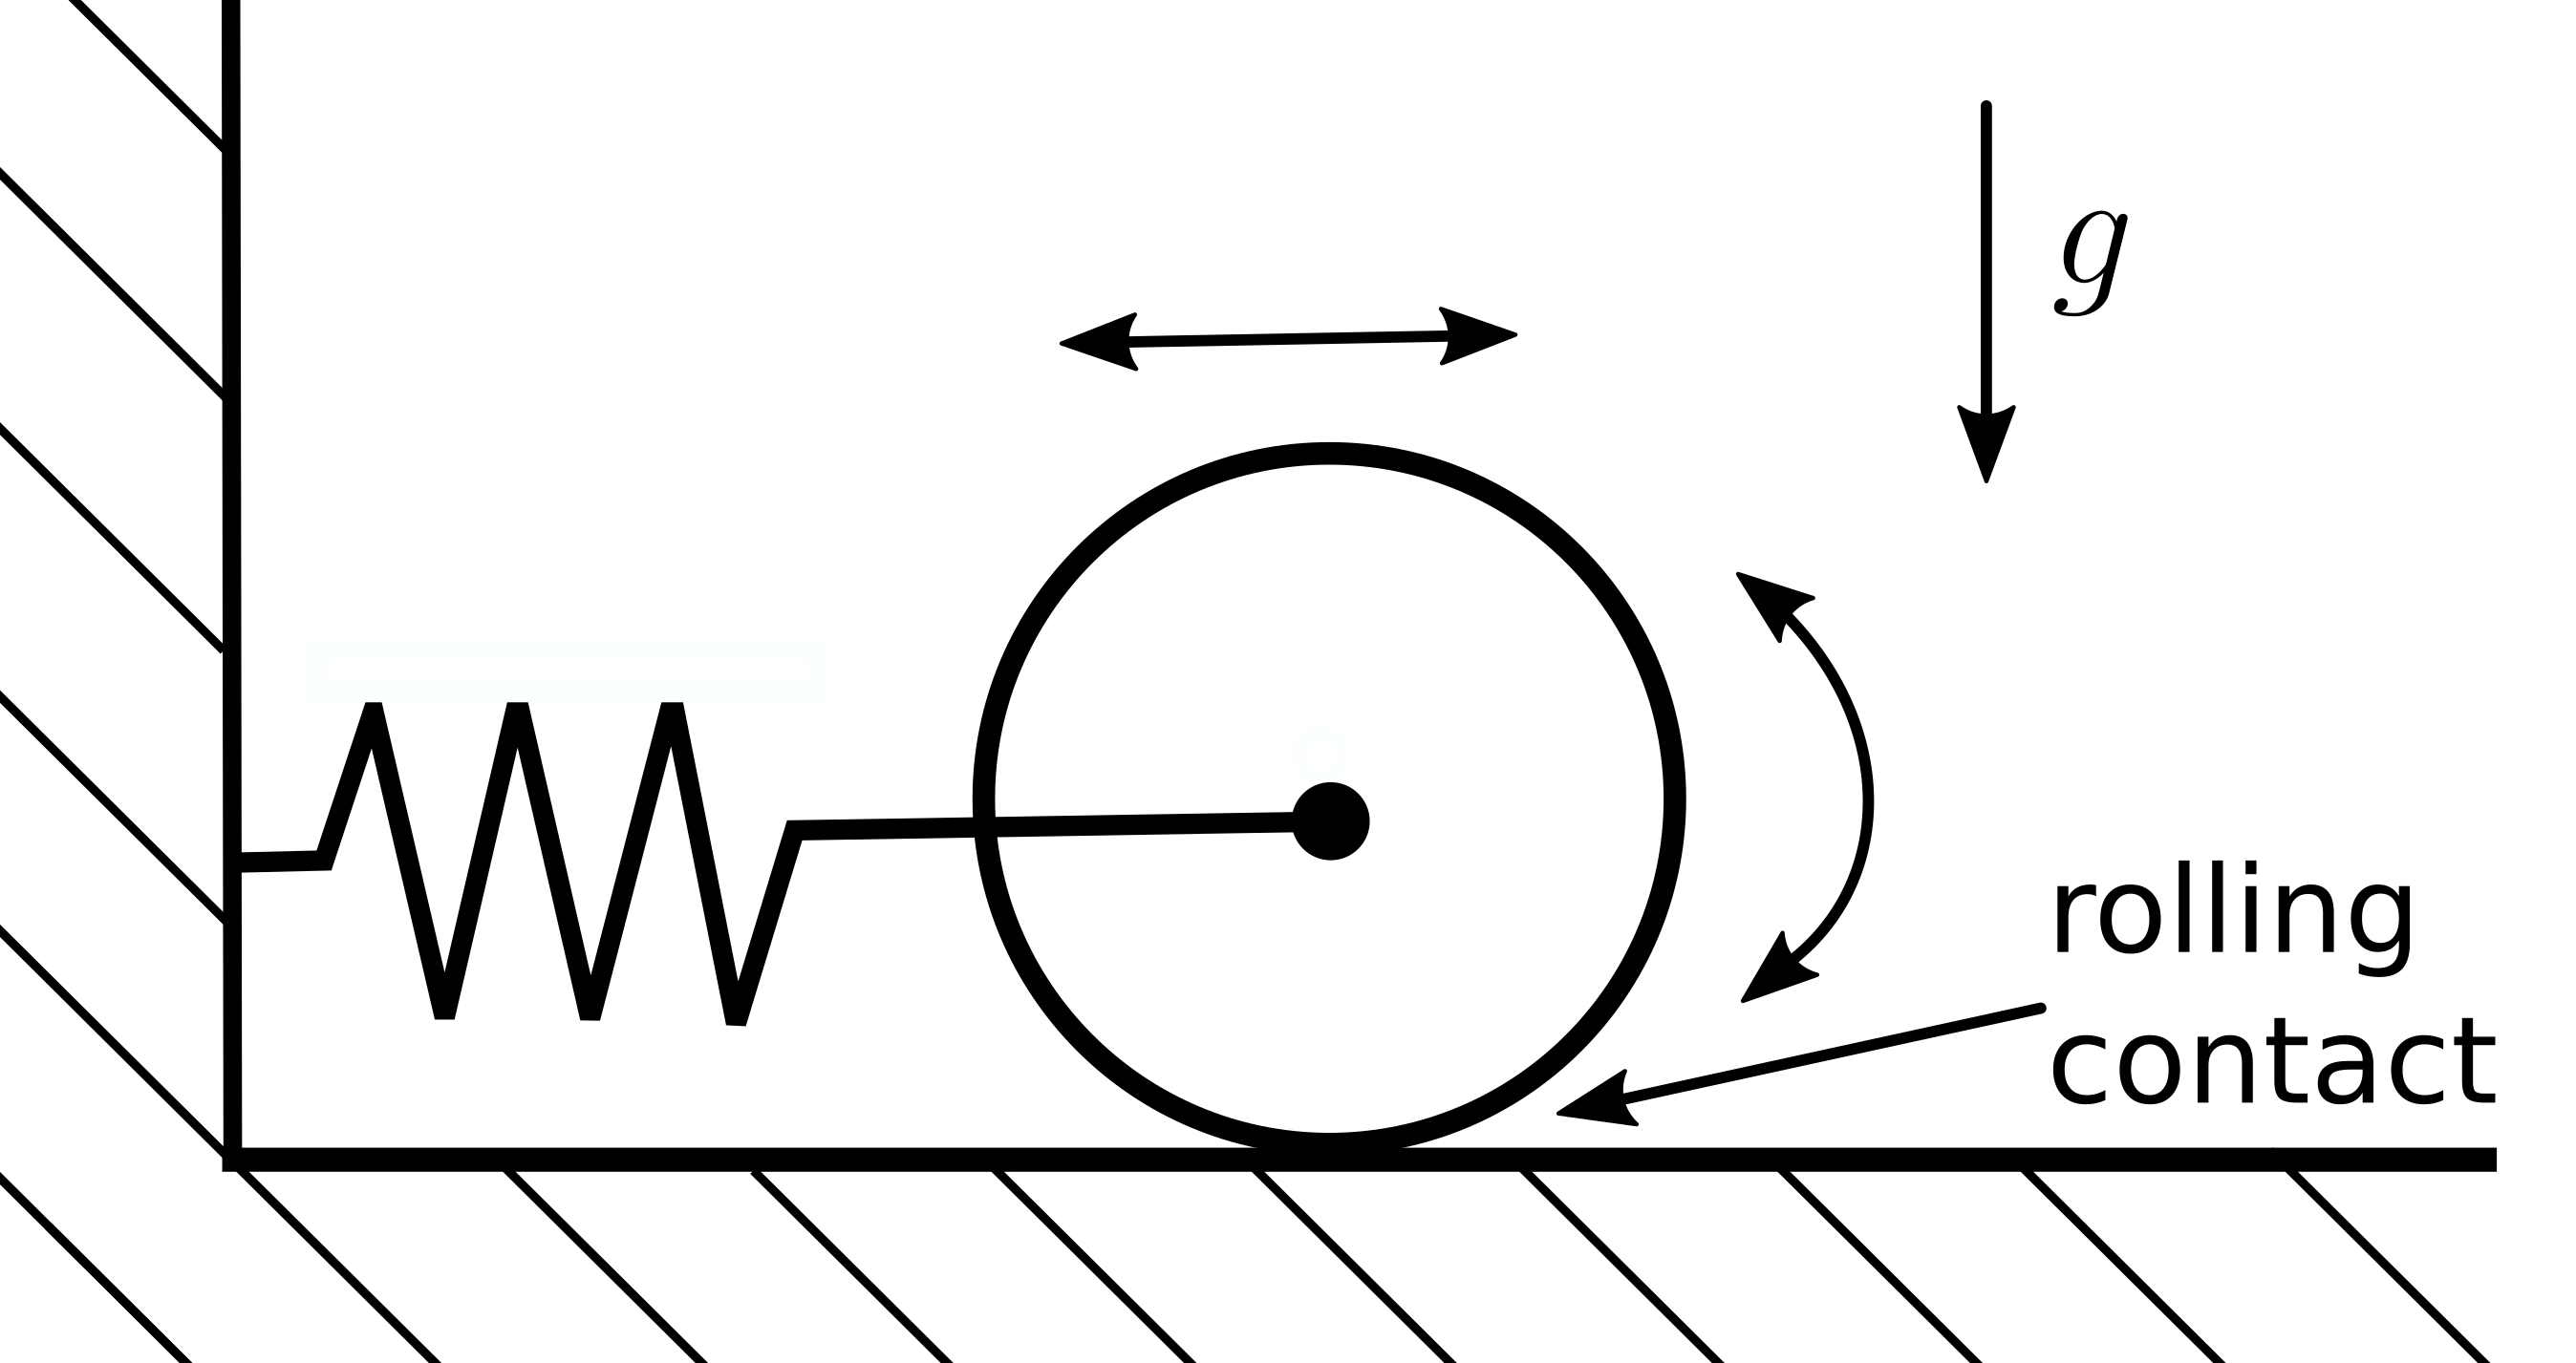
\includegraphics[width=0.6\columnwidth]{figures/schematics/spring_cylinder.png}
	\caption{\label{fig:spring_cylinder} 
	Spring-Cylinder system. The cylinder can translate horizontally and rotate.
	Friction with the ground establishes a non-dissipative rolling contact.}
\end{figure}

For reference, we first simulate this setup with frictionless contact, i.e.
$\mu=0$. Without friction, the cylinder does not rotate and we effectively have a
spring-mass system with natural frequency $\omega_n=\sqrt{k_s/m}$. We use a
rather coarse time step of $\delta t=0.02\text{ s}$, discretizing each period of
oscillation with about $22$ steps. Figure
\ref{fig:frictionless_spring_cylinder_energy} shows the total mechanical energy
as a function of time computed using three different schemes; symplectic Euler,
midpoint rule, and implicit Euler. The amount of numerical dissipation
introduced by the implicit Euler scheme dissipates the initial energy in just a
few periods of oscillation. For the symplectic Euler scheme, we observe in Fig.
\ref{fig:frictionless_spring_cylinder_energy} that, while the energy is not
conserved, it stays bounded, within a band 28\% peak-to-peak wide. The figure
also confirms that the second order midpoint scheme conserves energy exactly. These are well known theoretical properties of these
integration schemes when applied to the spring-mass system.
\begin{figure}[!h]
    \centering
    %trim={<left> <lower> <right> <upper>}
    \adjincludegraphics[width=0.49\columnwidth,trim={0 0 {0.05\width} 0},clip]{figures/spring_cylinder/frictionless_total_energy.png}
    \adjincludegraphics[width=0.49\columnwidth,trim={0 0 {0.05\width} 0},clip]{figures/spring_cylinder/frictionless_total_energy_long_term.png}    
    \caption{\label{fig:frictionless_spring_cylinder_energy} 
    Total mechanical energy for the frictionless spring-cylinder system in the
    first few periods of oscillation (left) and long term (right).}
\end{figure}

We now focus our attention to a case with frictional contact using $\mu=1$. As
we release the cylinder from its initial position at $x_0=0.1\text{ m}$,
friction with the ground establishes a rolling contact, and the system sets into
a periodic motion. Since now kinetic energy is split into translational and
rotational components, the rolling cylinder behaves as a spring-mass system with
an effective mass $m_\text{eff}=m+I_o/R^2$, with $I_o$ the rotational inertia of
the cylinder about its center. Therefore the frequency of oscillation is slower
and the same time step, $\delta t=0.02\text{ s}$, now discretizes one
period of oscillation with about 27 steps.

Total energy is shown in Fig. \ref{fig:spring_cylinder_energy}. Solutions computed with the implicit
Euler and the symplectic Euler schemes show similar trends to those in the frictionless
case. The midpoint rule does not conserve energy exactly, but it does
significantly better with a peak-to-peak variation of only 0.16\%. While the
ideal rolling contact does not dissipate energy, the regularized model of
friction does dissipate energy given the slip velocity is never exactly zero,
though small in the order of $\sim\sigma\mu\delta t g$ as shown in Section
\ref{sec:physical_intuition}. The symplectic Euler scheme and the midpoint rule
take $10$ minutes of simulated time and about $1000$ oscillations to dissipate
10\% of the total energy (Fig. \ref{fig:spring_cylinder_energy}, right). This
level of numerical dissipation is remarkably low, considering that real mechanical systems often introduce several sources of dissipation.
\begin{figure}[!h]
    \centering
    %trim={<left> <lower> <right> <upper>}
    \adjincludegraphics[width=0.49\columnwidth,trim={0 0 {0.05\width} 0},clip]{figures/spring_cylinder/total_energy.png}
    \adjincludegraphics[width=0.49\columnwidth,trim={0 0 {0.05\width} 0},clip]{figures/spring_cylinder/total_energy_long_term.png}    
    \caption{\label{fig:spring_cylinder_energy} 
    Total mechanical energy for the spring-cylinder system with friction $\mu=1$
    in the first few periods of oscillation (left) and long term (right).}
\end{figure}

To study the order of accuracy of our approach, we define the $L^2$-norm position error as
\begin{equation*}
    e_q = \left(\frac{1}{T}\int_0^T dt(x(t)-x_e(t))^2\right)^{1/2}
\end{equation*}
where $x_e(t)$ is the known exact solution. We simulate for $T=5\text{
s}$, about 10 periods of oscillation. Figure \ref{fig:spring_cylinder_position_error} shows the position error as
a function of the time step. We see that even with frictional contact, the two-stage approach
with the midpoint rule achieves second order of accuracy. Both the implicit Euler and the symplectic Euler schemes are first order,
though the error is significantly smaller when using the symplectic Euler
scheme.
\begin{figure}[!h]
	\centering
	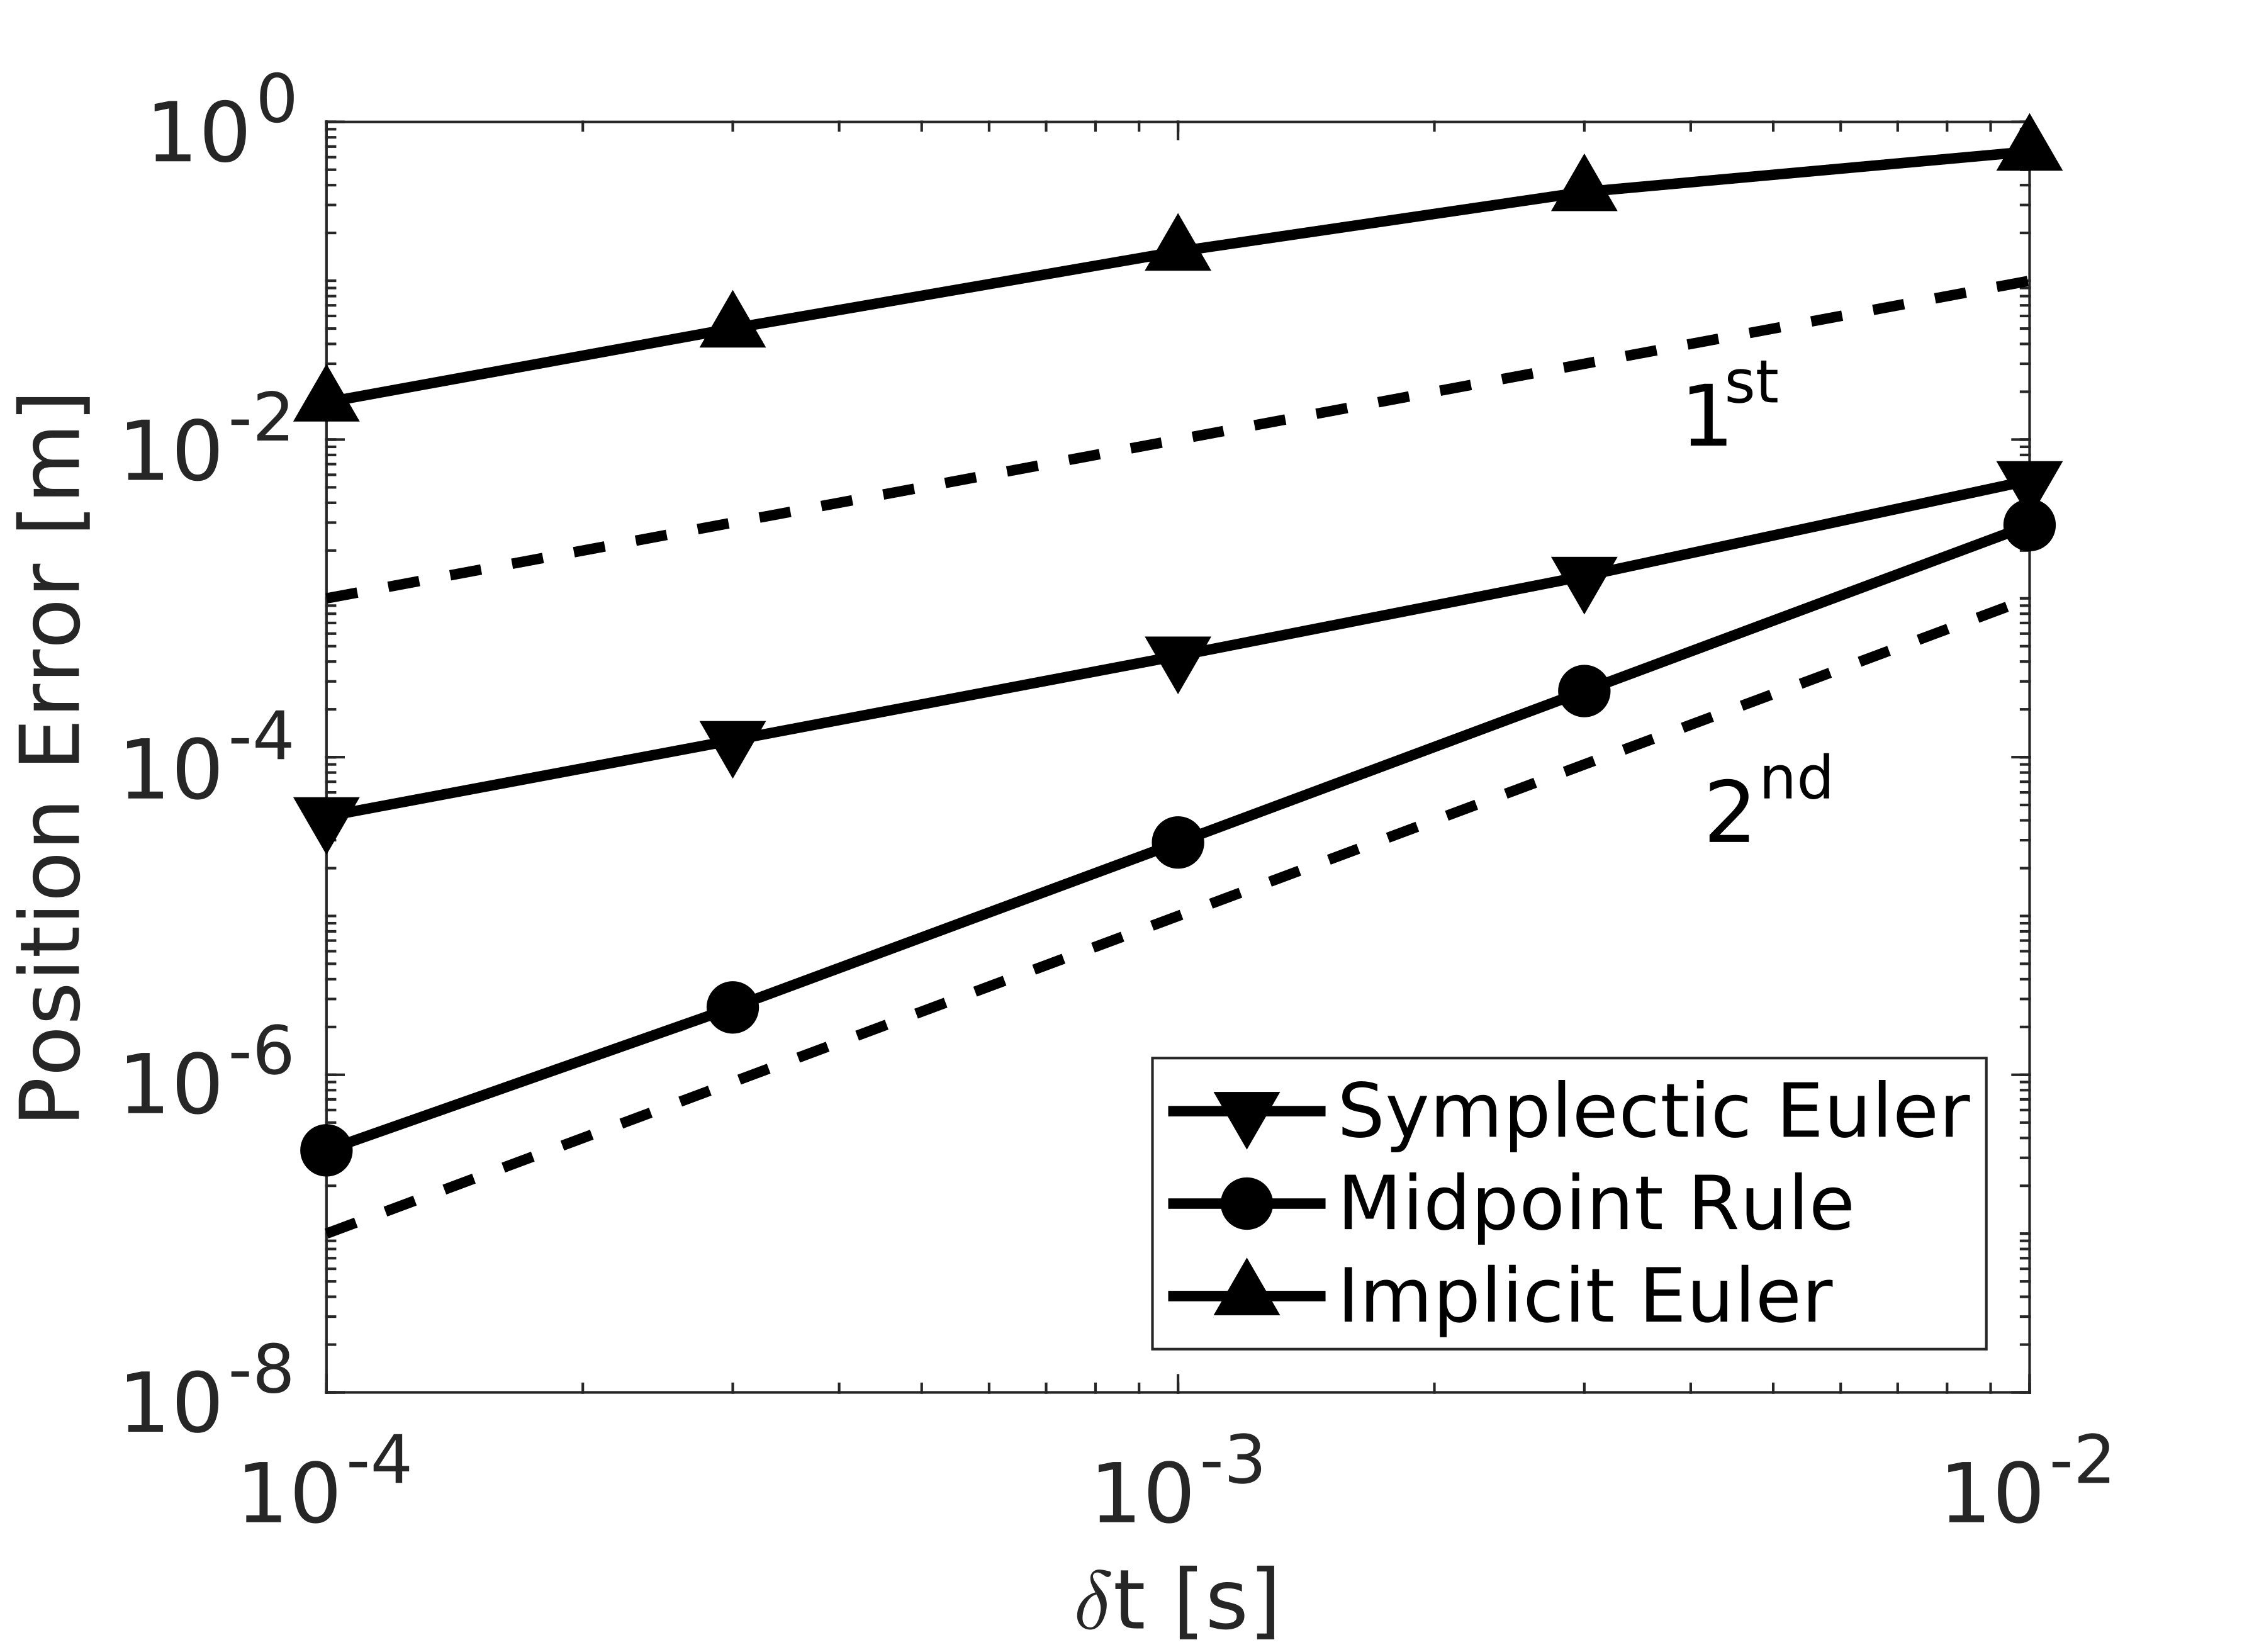
\includegraphics[width=0.7\columnwidth]{figures/spring_cylinder/position_error.png}
	\caption{\label{fig:spring_cylinder_position_error} 
	Position error as a function of time step for the spring-cylinder system
	with friction. First and second order references are shown with dashed
	lines.}
\end{figure}

\subsection{Clutter}
\label{sec:clutter}
The purpose of this case is to evaluate robustness, convergence properties, and
scalability of our SAP solver when compared against other existing methods.

The setup consists of an open container with a square base of size
$80~\text{cm}\times80~\text{cm}$ and $80~\text{cm}$ in height. Bodies are
dropped into this container in four different columns with the same number of
bodies each (see Fig. \ref{fig:clutter_snapshots}). Each column consists of an
arbitrary assortment of spheres of radius $5~\text{cm}$ and boxes with sides of
$10~\text{cm}$ in length. All bodies have density $1000\text{
kg}/\text{m}^3$ and therefore each sphere has a mass of approximately
$0.524\text{ kg}$ and each box has a mass of $1.0\text{ kg}$. We set a very high
contact stiffness of $k=10^{12}\text{ N}/\text{m}$ so that the model is in the
\emph{near-rigid} regime. The dissipation time scale is set to equal the time
step and the friction coefficient of all surfaces is $\mu=1.0$.
\begin{figure}[t]
    \centering
    %trim={<left> <lower> <right> <upper>}
    \adjincludegraphics[width=0.49\columnwidth,trim={0 {0.05\height} 0 0},clip]{figures/clutter/clutter_w_walls_t0.png}
    \adjincludegraphics[width=0.49\columnwidth,trim={0 {0.05\height} 0 0},clip]{figures/clutter/clutter_no_walls_t0.png}\\
    \vspace{0.1cm}
    \adjincludegraphics[width=0.49\columnwidth,trim={0 {0.05\height} 0 0},clip]{figures/clutter/clutter_w_walls_t2_zoom.png}
    \adjincludegraphics[width=0.49\columnwidth,trim={0 {0.05\height} 0 0},clip]{figures/clutter/clutter_no_walls_t2_zoom.png}
    \caption{Initial conditions (top) and an intermediate configuration after $2$ seconds of
    simulated time (bottom) for the clutter setup with (left) and without
    (right) walls. Many of the spheres in the configuration with no walls
	roll outside the frame in the intermediate configuration.}
    \label{fig:clutter_snapshots}
\end{figure}

We first run our simulations with 10 bodies per column for a total of 40 bodies.
We simulate 10 seconds using time steps of size $\delta t = 10\text{ ms}$.
Number of solver iterations and wall-clock time per time step are reported in
Fig. \ref{fig:clutter_w_walls_nb40} for the three solvers. We observe that SAP
needs to perform a larger number of iterations during the very energetic initial
transient. As the system reaches a steady state, however, SAP warm starts very
effectively, performing only about $3$ iterations per time step. Even though
SAP necessities a larger number of iterations to converge than Geodesic IPM during this initial transient, the wall-clock time per time step is very
similar. This tells us that SAP's cost per iteration is lower than that of
Geodesic IPM, even when they both use the same supernodal algebra. Unlike SAP and Geodesic IPM that benefit from warm start, we see that Gurobi performs
about $9$ iterations per time step in both the initial transient and the steady state.
\begin{figure}[!h]
	\centering
    %trim={<left> <lower> <right> <upper>}
    \adjincludegraphics[width=0.49\columnwidth,trim={0 0 0 0},clip]{figures/clutter/iterations_nb40.png}
    \adjincludegraphics[width=0.49\columnwidth,trim={0 0 0 0},clip]{figures/clutter/wall_clock_nb40.png}    
	\caption{\label{fig:clutter_w_walls_nb40} 
	Iterations and wall-clock time per time step for SAP, Geodesic IPM, and
	Gurobi for the clutter case with 40 bodies and with walls. Most of the
	energy is lost during the first $\sim300$ time steps as the objects pile up
	at the bottom of the box.}
\end{figure}

Figure \ref{fig:clutter_line_search} shows two examples of convergence history
for the case with walls. We denote with $\ell^0$ to the cost evaluated at the
initial guess, the previous time step velocity. With $\ell_*$ we denote the
optimal cost, which we approximate with its value from the last iteration. At
step 60 during the initial transient for which SAP requires 21 iterations to
converge, we observe that the algorithm reaches quadratic convergence after an
initial linear convergence transient. At step 520, past the initial energetic
transient, SAP exhibits linear convergence and satisfies the convergence
criteria within 5 iterations. We observed this convergence behavior for other
time steps as well. For time steps requiring about 10 iterations or more, SAP
exhibits linear convergence followed by quadratic convergence. For time steps
requiring less than about 10 iterations, the linear convergence regime is enough
to reach convergence.
\begin{figure}[!h]
	\centering
    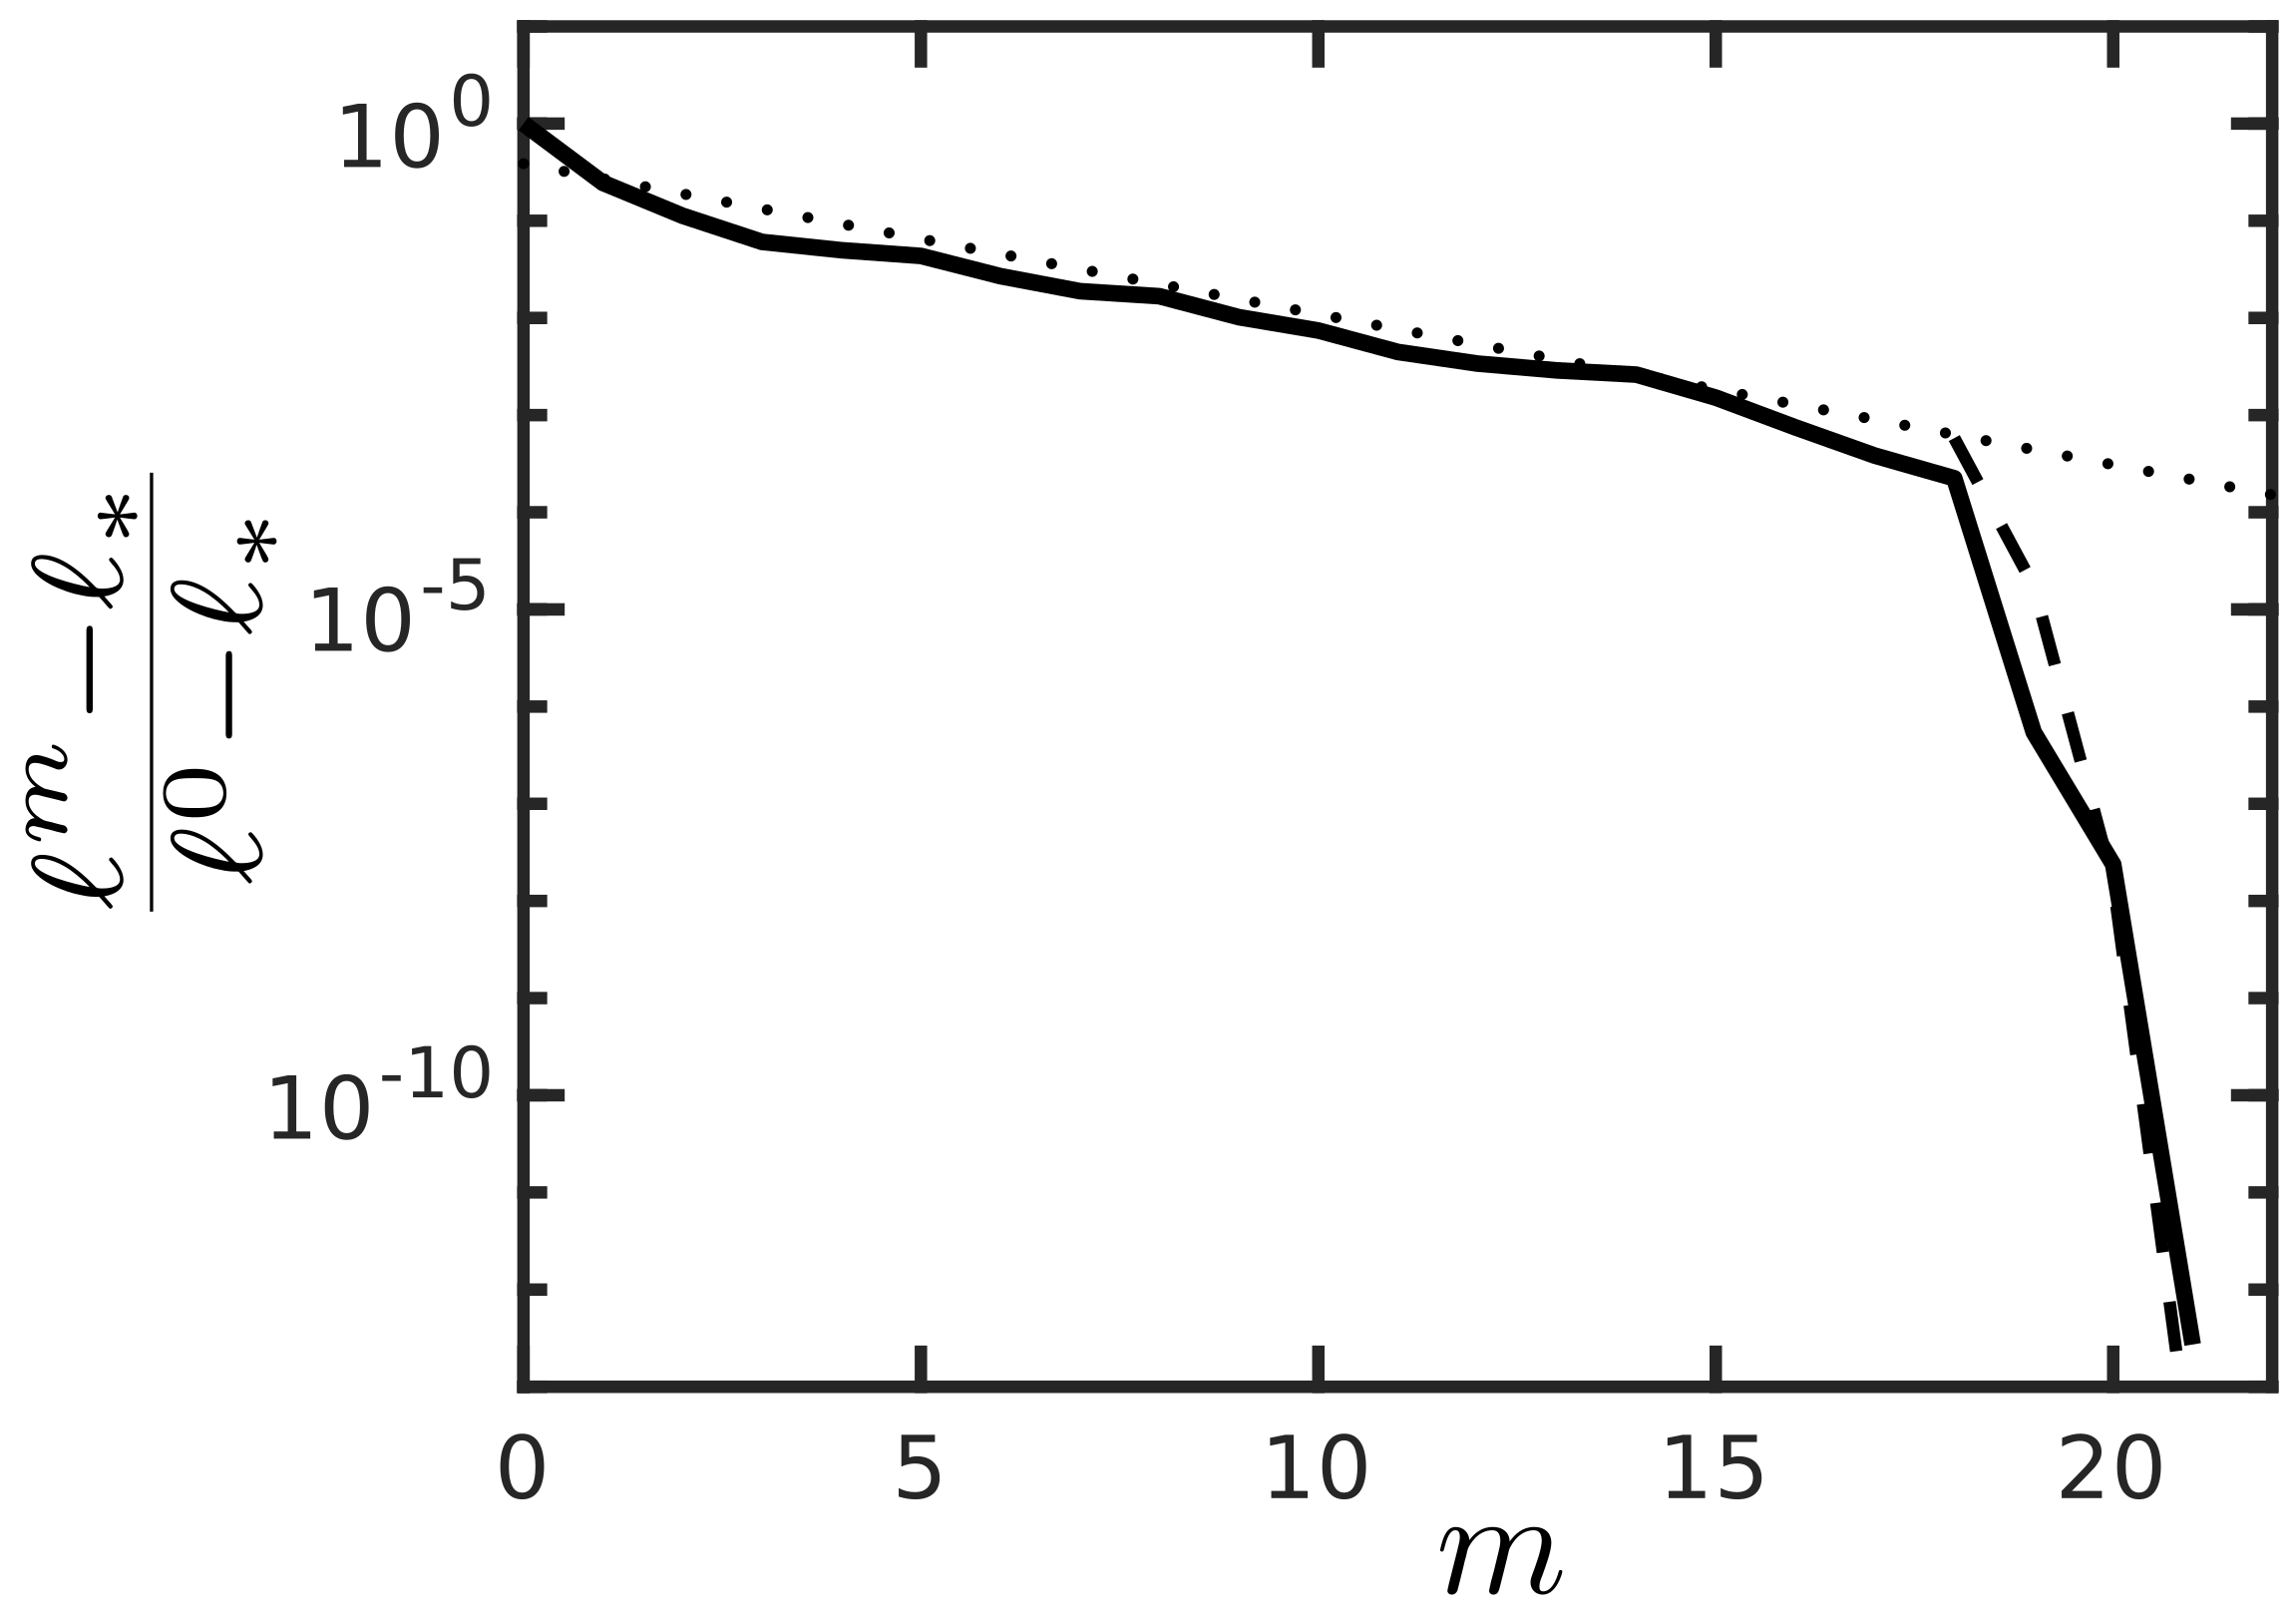
\includegraphics[height=0.34\columnwidth]{figures/clutter/normalized_cost_step60_21its_wwalls_latex_labels.png}
	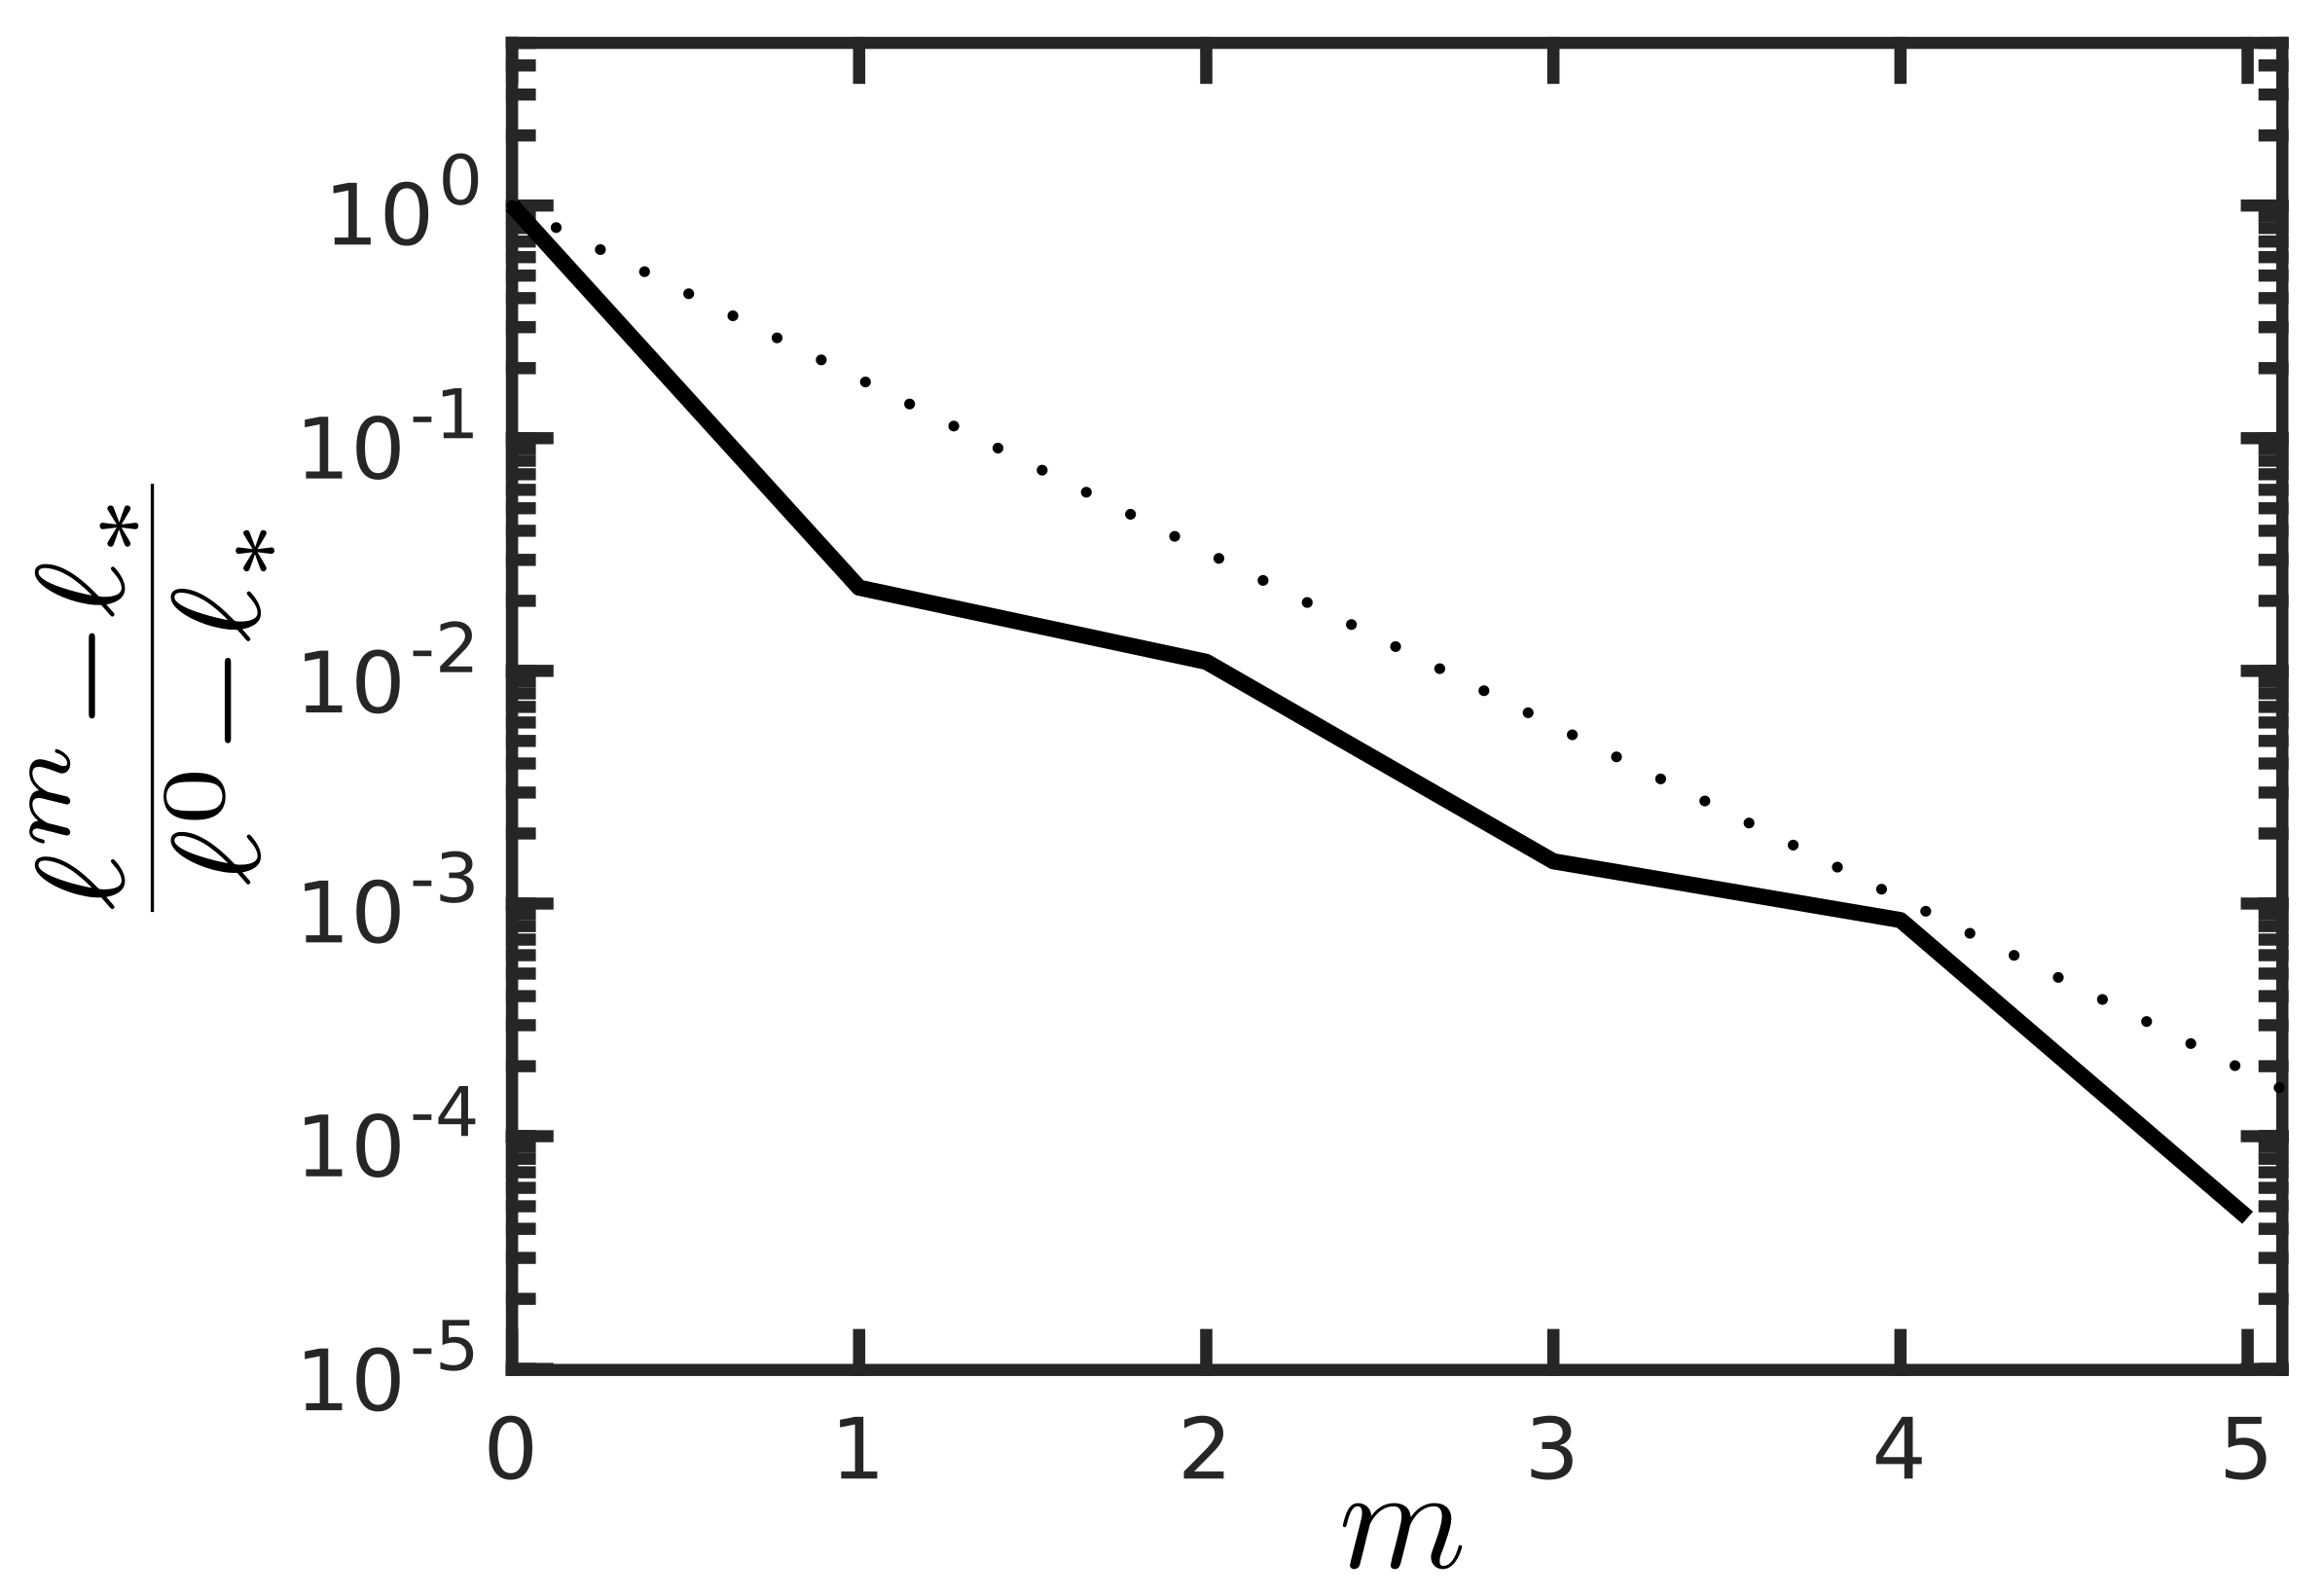
\includegraphics[height=0.34\columnwidth]{figures/clutter/normalized_cost_step520_5its_wwalls_latex_labels.png}    
	\caption{\label{fig:clutter_line_search} 
	Normalized cost as a function of Newton iterations for step 60 (left) and for step 520 (right). SAP ensures that the cost decreases with each newt iteration. Reference lines are shown for linear convergence (dotted) and quadratic convergence (dashed).}
\end{figure}

\subsubsection{Scalability}

We evaluate the performance of SAP with different problem sizes by varying the
number of objects in the clutter with all other parameters held constant. We
study scalability of the test case both with and without walls (see
Fig. \ref{fig:clutter_snapshots}) as the variation in the setup leads to very
different sequences of contact configuration. The size of the problems can be
appreciated in Fig. \ref{fig:clutter_num_contats} showing the number of contact
constraints at the end of the simulation when objects are in steady state
against the number of objects. We observe a larger number of contacts for the
configuration without walls since in this configuration many of the boxes spread
over the ground and lay flat on one of their faces, leading to a multi-contact
configuration (see Fig. \ref{fig:clutter_snapshots} for instance). Notice that
each body contributes 6 DOFs and each contact constraint contributes 3 unknowns.
Therefore, in the case with 200 bodies, the problem involves 1200 DOFs and about
2700 contact unknowns for a total of about 3000 unknowns.
\begin{figure}[!h]
	\centering
	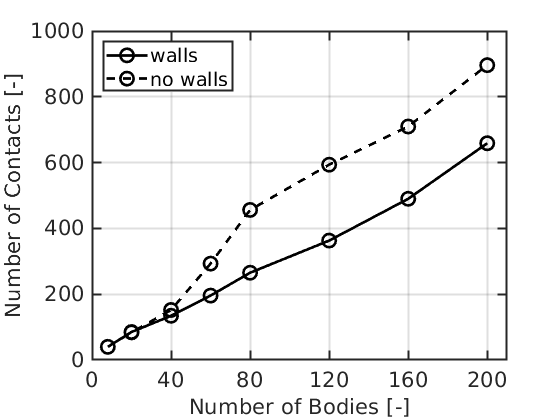
\includegraphics[width=0.7\columnwidth]{figures/clutter/number_of_contacts.png}
	\caption{\label{fig:clutter_num_contats} 
	Total number of contacts with objects in steady state at the end of the
	simulation for setup with and without walls.}
\end{figure}

We measure the total time spent by each solver and define the \emph{speedup}
against Gurobi. Figure \ref{fig:clutter_speedup} shows the speedup for both
SAP and Geodesic IPM in the configuration with and without walls.
The setup with walls is particularly difficult given that objects are
constrained to pile up, leading to a configuration in which almost all objects
are coupled with every other object by frictional contact
(see Fig. \ref{fig:clutter_snapshots}). That is, the motion of an object at the
bottom of the pile can lead to motion of another object far on top of the pile.
In contrast, the simulation with no walls leads to \emph{islands} of objects
that do not interact with each other.

In general, we observe two regimes. For problems with less than about 40 bodies,
SAP outperforms Gurobi significantly by up to a factor of 25 in the case with
walls and up to a factor of 50 with no walls. Beyond 80 bodies, Gurobi
outperforms both SAP and Geodesic IPM in the case with walls, but SAP is about
10 times faster for the case with no walls. Though SAP shows to be about twice
as fast as Geodesic IPM for most problem sizes, it can be five times faster for
small problems with 8 bodies or less.
\begin{figure}[!h]
	\centering
    %trim={<left> <lower> <right> <upper>}
    \adjincludegraphics[width=0.49\columnwidth,trim={{0.02\width} 0 {0.05\width} 0},clip]{figures/clutter/speedup_w_walls.png}
    \adjincludegraphics[width=0.49\columnwidth,trim={{0.02\width} 0 {0.05\width} 0},clip]{figures/clutter/speedup_no_walls.png}
	\caption{\label{fig:clutter_speedup} 
	Speedup against Gurobi for both SAP and Geodesic IPM for the configuration with walls (left) and without walls (right).}
\end{figure}

It could be argued that these speedup results depend on the accuracy settings of
each solver. For a fair comparison, we define the dimensionless momentum error
as
\begin{equation}
	e_m = \frac{\Vert\tilde{\nabla}\ell_p\Vert}{\max(\Vert\tilde{\mf{p}}\Vert,\Vert\tilde{\mf{j}_c}\Vert)},
	\label{eq:momentum_error}
\end{equation}
using the scaled generalized momentum quantities in Eq.
(\ref{eq:scaled_momentum_quantities}). We also define the dimensionless
complementarity slackness error as
\begin{equation}
	e_\mu = \frac{1/n_c\sum_i|\bm{g}_i\cdot\bgamma_i|}{\ell_p}.
	\label{eq:slackness_error}
\end{equation}

Figure \ref{fig:clutter_errors_w_wall} shows average values of $e_m$ and $e_\mu$
over all time steps. Since SAP satisfies the complementarity slackness exactly,
$e_\mu$ is not shown. We have verified this to be true within machine precision
for all simulated cases.

SAP's momentum error is below $10^{-5}$ as expected since this is the value used
for the termination condition. Similarly, the complementarity slackness is below
$10^{-5}$ for Geodesic IPM, since this is the value used for its own termination
condition. Gurobi does a good job at satisfying the complementarity slackness.
However, it is the solver with the largest error in the momentum equations, even
though both SAP and Geodesic IPM outperform Gurobi in most of the test cases.
These metrics demonstrate that when SAP and Geodesic IPM outperform Gurobi, it
is not at the cost of losing accuracy.
\begin{figure}[!h]
	\centering
    %trim={<left> <lower> <right> <upper>}
    \adjincludegraphics[height=0.40\columnwidth,trim={0 0 {0.05\width} 0},clip]{figures/clutter/momentum_error_w_walls.png}
	\adjincludegraphics[height=0.40\columnwidth,trim={{0.05\width} 0 {0.05\width} 0},clip]{figures/clutter/momentum_error_no_walls.png}\\
    \adjincludegraphics[height=0.40\columnwidth,trim={0 0 {0.05\width} 0},clip]{figures/clutter/optimality_condition_error_w_walls.png}
    \adjincludegraphics[height=0.40\columnwidth,trim={{0.05\width} 0 {0.05\width} 0},clip]{figures/clutter/optimality_condition_error_no_walls.png}
	\caption{\label{fig:clutter_errors_w_wall} 
	Momentum balance error $e_m$ (top) and complementarity condition error
	$e_\mu$ (bottom) for the clutter case with walls (left) and without walls
	(right).}
\end{figure}

\subsubsection{Slip Parameter}

We study the effect of the slip parameter $\sigma$ in Eq.
(\ref{eq:slip_time_scale}). As before, we use $\delta t = 10\text{ ms}$ and
simulate 40 objects for 10 seconds to a steady state configuration. At this
steady state at the end of the simulation, we compute the mean slip velocity
among all contacts. Figure \ref{fig:clutter_sigma_vt} shows this mean slip
velocity along with the estimated slip in Eq. (\ref{eq:slip_estimation}), $v_s
\approx\sigma\mu\delta t g$, shown in dashed lines. We see that the mean slip
velocity remains below the estimated slip as expected in a static configuration
with objects in stiction. In the case with walls where stiction helps to hold
the steady state static configuration, we see that the mean slip velocity
closely follows the slope of the slip estimate. Without the walls, objects do
not pile up in a complex static structure but simply lie on the ground, and
therefore, the resulting slip velocities are significantly smaller. The sudden
drop in the slip velocity for $\sigma>10^{-3}$ is caused by the sensitivity of
the final state on the value of $\sigma$. As $\sigma$ increases, so does the
slip velocity bound $v_s$ and objects in the configuration without walls can
slowly drift into a configuration leading to more contacts. In particular, boxes
are more likely to slowly drift until one of their faces lies flat
on the ground, a configuration with zero slip once steady state is reached.
Finally, we observe that when using $\sigma=10^{-3}$, the amount of slip is
negligible for robotic applications.
\begin{figure}[!h]
	\centering
	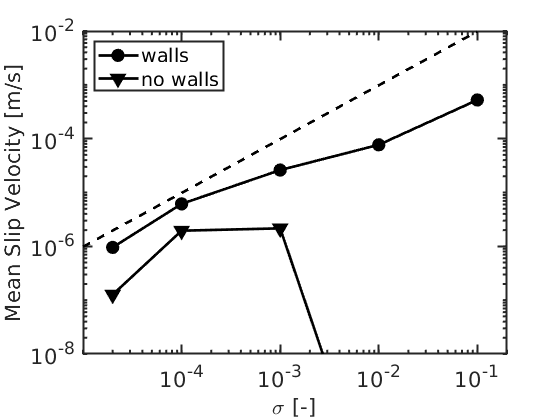
\includegraphics[width=0.7\columnwidth]{figures/clutter/sigma_vt.png}
	\caption{\label{fig:clutter_sigma_vt} 
	Mean slip velocity at the end of the simulation with objects at rest as a
	function of the slip parameter. The estimated slip $v_s = \sigma\mu\delta t g$ is shown in dashed lines.}
\end{figure}

We conclude by examining the effect of $\sigma$ on the conditioning of the
system. Figure \ref{fig:clutter_sigma} shows the condition number of the Hessian
in the final configuration and the mean number of Newton iterations throughout
the simulation. We see that the condition number scales as $\sigma^{-1}$ while
the mean number of Newton iterations is roughly proportional to  $\ln(\sigma)$.
Notice that our choice $\sigma=10^{-3}$ for this paper is placed right in the
middle, in a log scale, of the range of values examined in this study.
\begin{figure}[!h]
	\centering
    %trim={<left> <lower> <right> <upper>}
    \adjincludegraphics[width=0.49\columnwidth,trim={0 0 {0.05\width} 0},clip]{figures/clutter/sigma_iterations.png}
    \adjincludegraphics[width=0.49\columnwidth,trim={0 0 {0.05\width} 0},clip]{figures/clutter/sigma_condition_number.png}
	\caption{\label{fig:clutter_sigma} 
	Effect of the slip parameter on the conditioning of the system. Mean Newton iterations per step (left) and mean condition number (right).}
\end{figure}


\subsection{Slip Control}
\label{sec:slip_control}
While previous work on convex approximations model rigid contact
\cite{bib:anitescu2006,bib:mazhar2014} or use regularization as a means of
constraint stabilization \cite{bib:todorov2014}, our work is novel in that we
incorporate physical compliance. This allows us not only to model compliant
point contact, but also to incorporate sophisticated models of surfaces patches.
We incorporate the pressure field model \cite{bib:elandt2019pressure}
implemented as part of Drake's \cite{bib:drake} \emph{hydroelastic contact}
model. We use the discrete approximation introduced in
\cite{bib:masterjohn2021discrete} to approximate each face of the contact
surface as a compliant element at its centroid.

To demonstrate this capability, we reproduce the test in
\cite{bib:masterjohn2021discrete} that models a \emph{Soft-bubble} gripper
\cite{bib:kuppuswamy2020soft}; a parallel jaw WSG 50 Schunk gripper outfitted
with air filled compliant surfaces. The aforementioned gripper is simulated
anchored to the world holding a spatula by the handle horizontally. We use
$\delta t=5\times 10^{-3}\text{ s}$. The grasp force is commanded to vary
between 1 N and 16 N with square wave having a 6 second period and a 75\% duty
cycle, left on Fig.~\ref{fig:slip_control_history}. \reviewquestion{R8-Q3}{This
results in a periodic transition from a secure grip to a loose grip allowing the
spatula to pitch in a controlled manner within grasp, see
Fig.~\ref{fig:slip_control_history} and the accompanying video. These contact
mode transitions are resolved by our model.} We observe that stiction during the
secure grip is properly resolved with the tight bounds for the slip due to
regularization discussed in Section \ref{sec:conditioning}.
While this case only has 8 degrees of freedom, it generates about 60 contact
constraints during the slip phase and about 160 contact constraints during the
stiction phase.

\begin{figure}[!h]
	\centering
	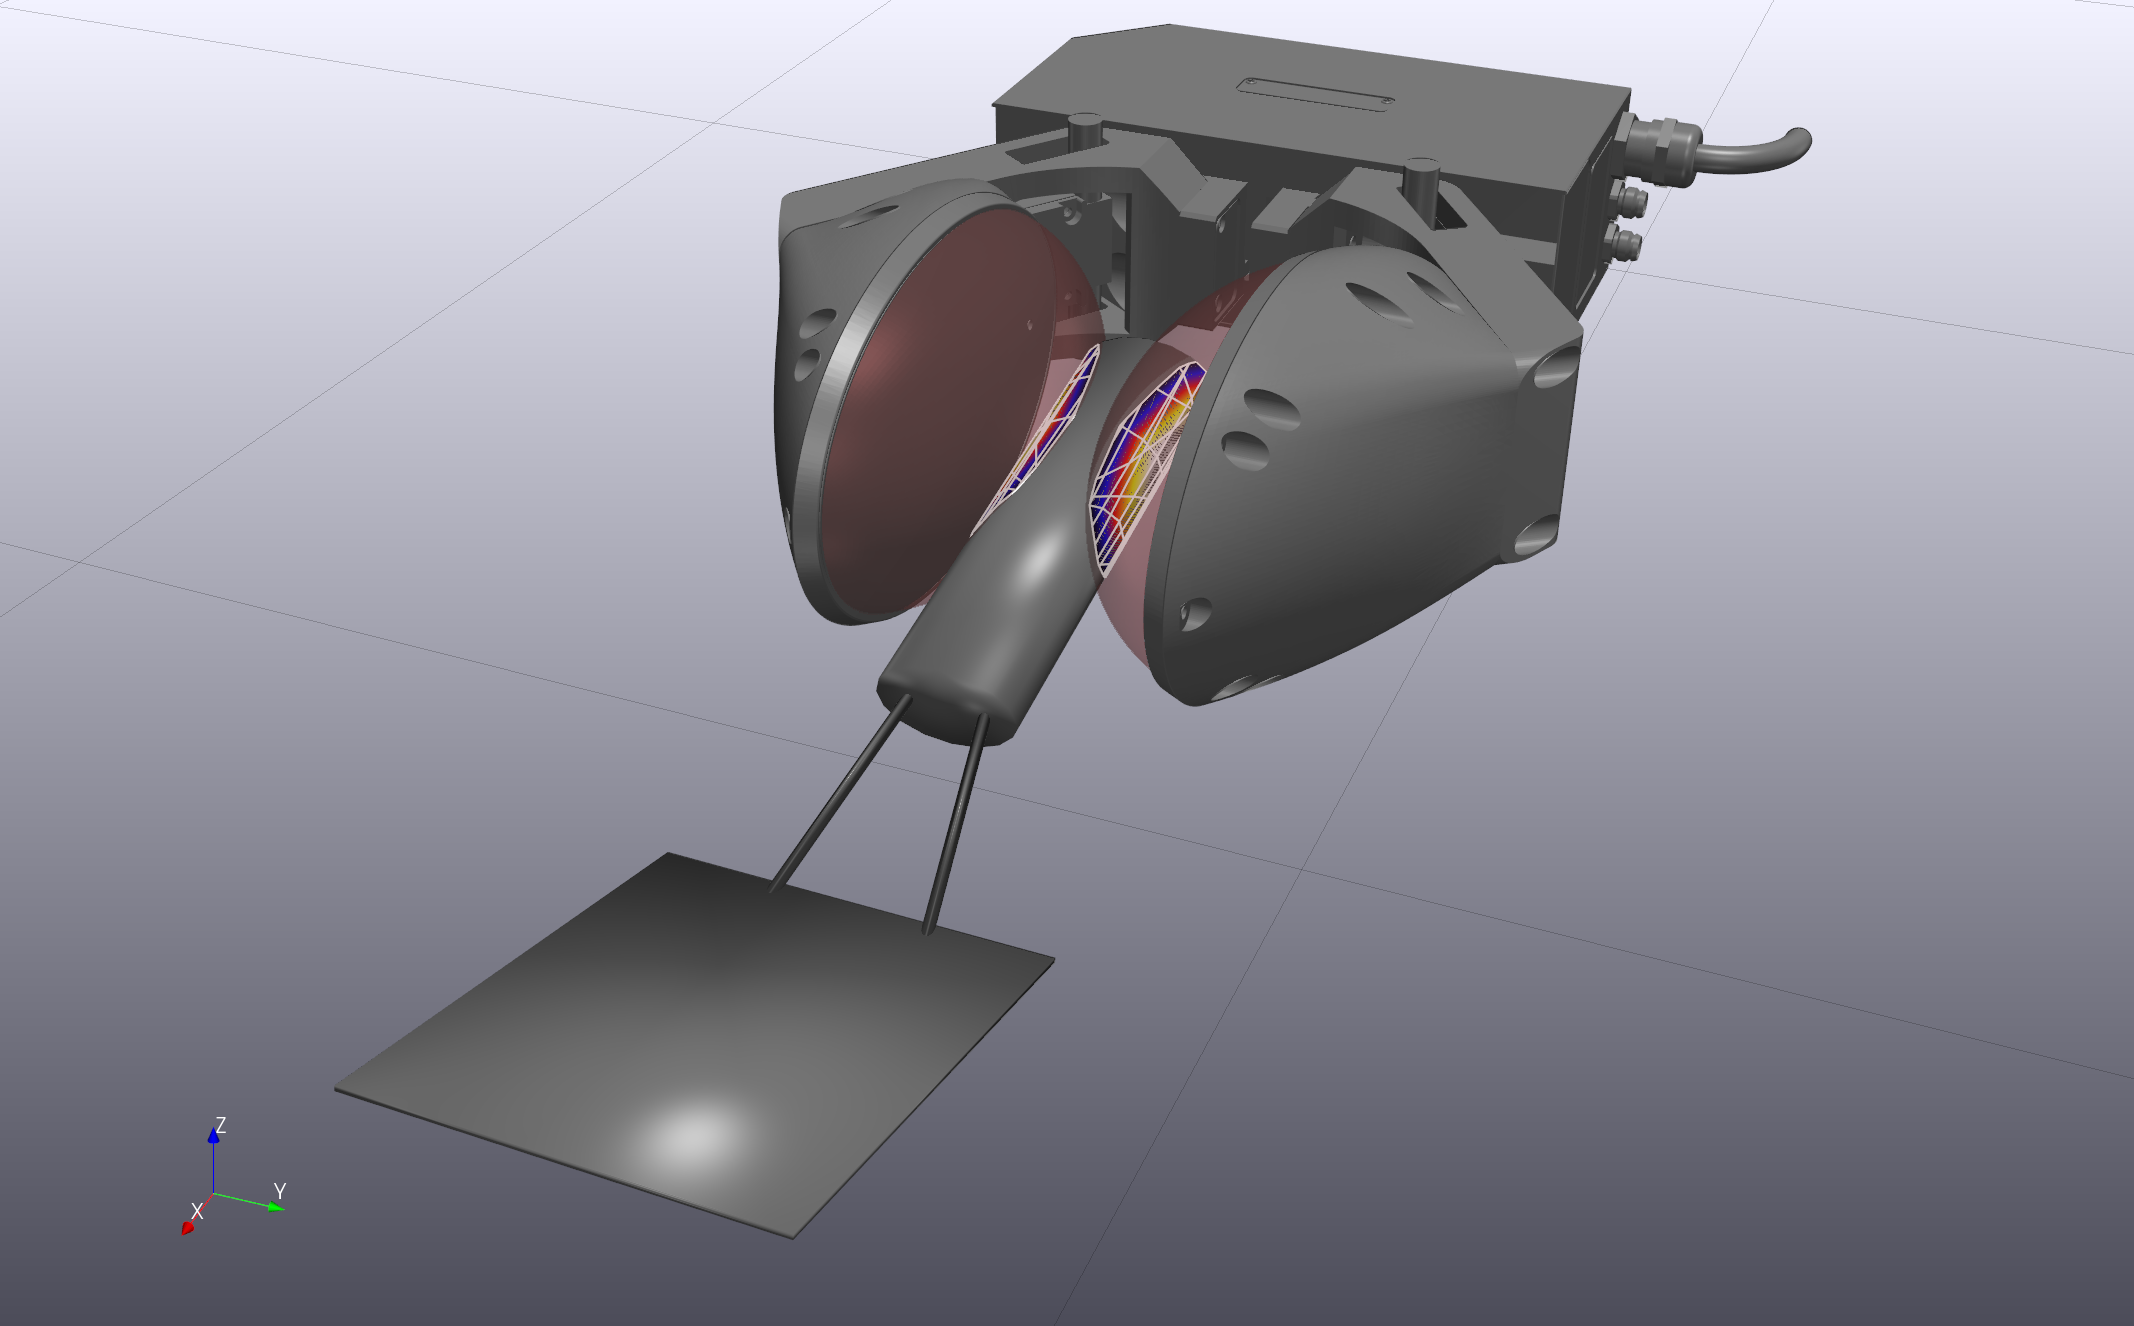
\includegraphics[width=0.8\columnwidth]{figures/slip_control/slip_control_single_frame.png}
	\caption{\label{fig:slip_control_frame} 
	Highly compliant \emph{Soft-bubble} gripper \cite{bib:kuppuswamy2020soft}
	holding a spatula. Unlike traditional point contact approaches, the
	hydroelastic contact model provides rich contact information and captures
	area-dependent phenomena such as the net-torque to hold the spatula. Contact
	patches are colored by contact pressure.}
\end{figure}

\begin{figure}[!h]
	\centering
    %trim={<left> <lower> <right> <upper>}
    \adjincludegraphics[width=0.49\columnwidth,trim={0 0 {0.05\width} 0},clip]{figures/slip_control/controller_force.png}
    \adjincludegraphics[width=0.49\columnwidth,trim={0 0 {0.05\width} 0},clip]{figures/slip_control/spatula_pitch.png}
	\caption{\label{fig:slip_control_history} 
	Grip force command (left) and spatula pitch angle (right) as a function of
	time.}
\end{figure}

We compare the performance of SAP against both Gurobi and Geodesic IPM, see
Section \ref{sec:about_solvers}. For SAP we use a relative tolerance
$\varepsilon_r=10^{-3}$, see Section \ref{sec:stopping_criteria}. For Gurobi we
set its tolerance parameter \verb+BarQCPConvTol+ to $10^{-8}$. For Geodesic IPM,
we set its complementary slackness tolerance to $10^{-6}$; larger values lead to
failure for this task. SAP bounds the momentum error, exhibiting a maximum value
of of $9.99\times 10^{-2}\,\%$. Even with such a tight tolerance, Gurobi
exhibits $2.6\,\%$ maximum error. Geodesic IPM's errors are significantly
smaller, below $2\times 10^{-4}\,\%$. However its robustness is very sensitive
to the specified tolerance.

Even though SAP's solutions are significantly more accurate than those from
Gurobi, it performs 92 times faster than Gurobi. SAP is 20 times faster than
Geodesic IPM and significantly more robust to solver tolerances. In terms of
solver iterations, SAP only performs 0.62 iterations on average, showcasing how
effectively it warm-starts. Geodesic IPM performs 5.6 iterations per step on
average and Gurobi performs 10.1 iterations on average.


\subsection{Dual Arm Manipulation}
\label{sec:dual_arm}
We demonstrate the effectiveness of our approach with the simulation of a
complex manipulation task. In this scenario, two Kuka IIWA arms (7 DOFs each)
are outfitted with anthropomorphic Allegro hands (16 DOFs each) (Fig.
\ref{fig:dual_arm_frames}). In front of the robot, a table has a jar (with a lid,
12 DOFs) full of 16 marbles of $50$~gr each (96 DOFs) and a bowl (6 DOFs),
completing the model with a total of 160 DOFs. Contact between the jar and the
lid is modeled using Drake's hydroelastic model \cite{bib:elandt2019pressure,
bib:masterjohn2021discrete} (see Section \ref{sec:slip_control}), while point
contact is used for all other interactions. The time step is set to $\delta
t=5\times 10^{-3}$~s.

The arms' controllers track a prescribed sequence of Cartesian end-effector
keyframe poses, while the hands' controllers track prescribed \emph{open/close}
configurations. We use force feedback to gauge successful grasps and to know
when the jar makes contact with the table. The robot is commanded to open the
jar, pour its contents into the bowl, close the lid and put the empty jar back
in place (keyframes in Fig. \ref{fig:dual_arm_frames} and the accompanying
video). 

This particular task generates hundreds of contact constraints, as shown in Fig.
\ref{fig:dual_arm_contacts} which also labels important events during the task.
\reviewquestion{R8-Q3}{We remark that our framework predicts contact mode
switching as a result of the computation. For instance, the lid initially
covering the jar is held by stiction and it transitions to sliding as the robot
pulls it out.}

\begin{figure}[!h]
	\centering
    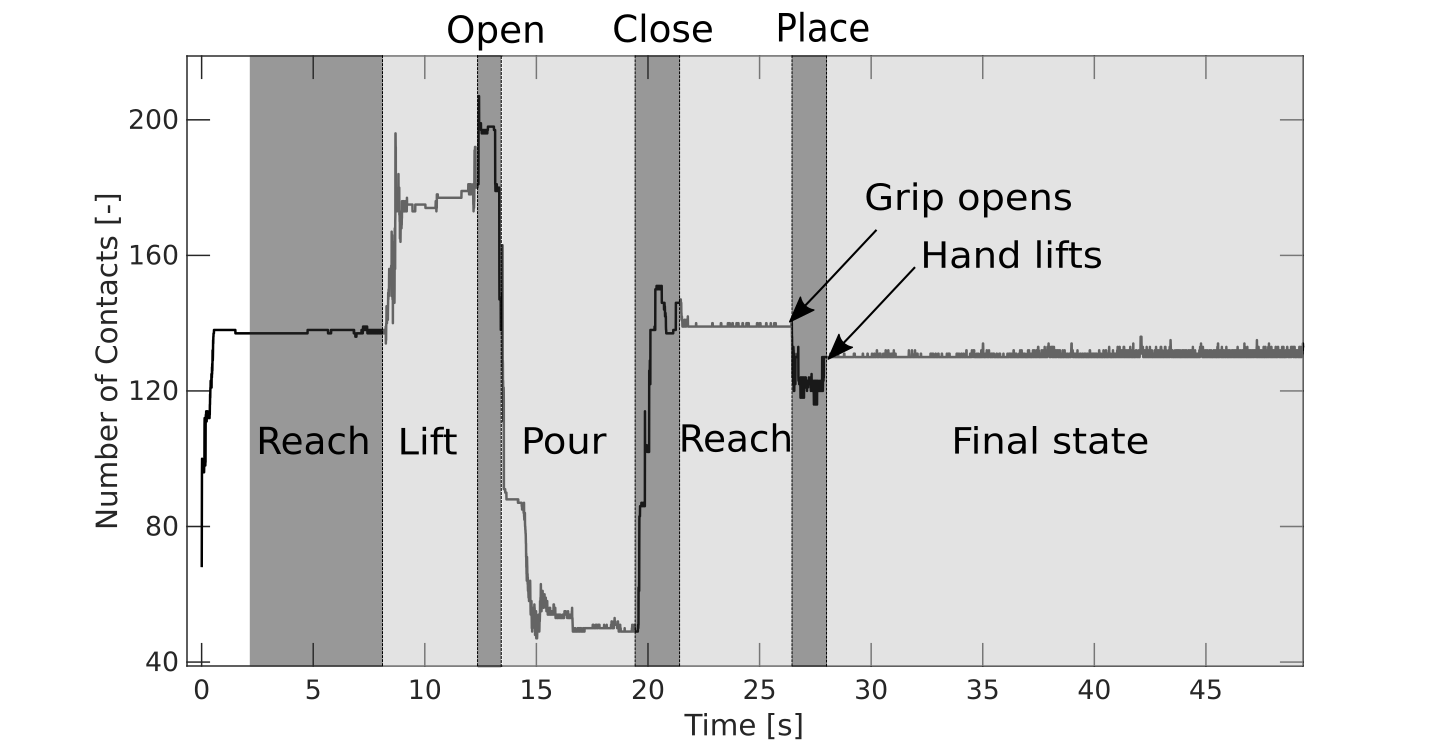
\includegraphics[width=0.9\columnwidth]{figures/dual_arm/dual_arm_contact.png}
    \caption{\label{fig:dual_arm_contacts} Number of contact constraints as a
    function time. Important events during the task are highlighted.}
\end{figure}

To assess accuracy, we evaluate the dimensionless momentum and complementarity
slackness errors defined in Eqs. \eqref{eq:momentum_error} and
\eqref{eq:slackness_error} respectively. We perform the simulation of the same
task several times using different solver tolerances. The results of these runs
are shown in Figures \ref{fig:dual_arm_momentum} and
\ref{fig:dual_arm_slackness}. Even though each solver uses a different tolerance
parameter, it is still useful to place these tolerances in the same horizontal
axis. The maximum tolerance we use for each solver corresponds to the largest
value that can be used to complete the task successfully. For Gurobi and
Geodesic IPM, smaller values of the tolerance parameter make the simulation
impractically slow. SAP on the other hand cannot achieve errors below $10^{-6}$
for this case due to round-off errors. Figures \ref{fig:dual_arm_momentum} and
\ref{fig:dual_arm_slackness} show both mean and median of the errors over the
entire simulation to show errors do not follow a symmetric distribution. More
interesting however are the minimum and maximum errors, shown as shaded areas.
SAP guarantees that momentum errors are below the specified tolerance, given
this is precisely its stopping criteria in Eq. \eqref{eq:stopping_criteria}. We
see however that it is difficult to correlate the expected error to solver
tolerance when using Gurobi or Geodesic IPM. In practice, we consistently
observe that the robot does not complete the task successfully when
momentum errors are larger than about $10\%$, regardless of the solver.
Therefore, we find that being able to specify a tolerance for the momentum
error directly is immensely useful. Given that SAP satisfies the complementarity
slackness condition exactly, complementarity slackness error for SAP is not
included in Fig. \ref{fig:dual_arm_slackness}.

\begin{figure}[!h]
	\centering
    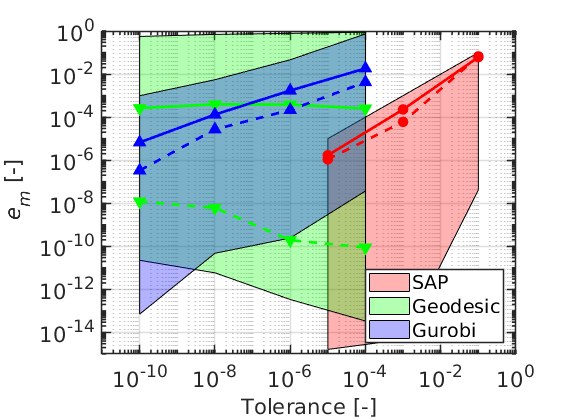
\includegraphics[width=0.7\columnwidth]{figures/dual_arm/momentum_error.png}
    \caption{\label{fig:dual_arm_momentum} Dimensionless momentum error, defined
    in Eq. \eqref{eq:momentum_error}. Mean (solid) and median (dashed) errors
    along with minimum and maximum errors (shaded areas) over the entire
    simulation.}
\end{figure}

\begin{figure}[!h]
	\centering
    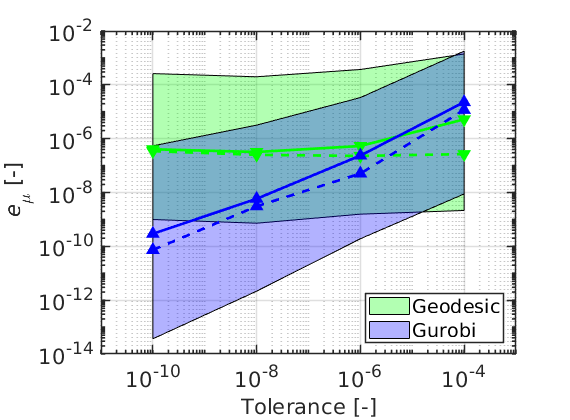
\includegraphics[width=0.7\columnwidth]{figures/dual_arm/optimality_condition.png}
    \caption{\label{fig:dual_arm_slackness} Dimensionless complementarity
    slackness error, defined in Eq. \eqref{eq:slackness_error}. Mean (solid) and
    median (dashed) errors along with minimum and maximum errors (shaded areas)
    over the entire simulation.}
\end{figure}

Figure \ref{fig:dual_arm_iterations} shows the mean number of iterations per
time-step for each solver. We see that the number of iterations needed by the
SAP solver is consistently below the other two solvers given how effectively SAP
warm-starts from the previous time-step solution.

To make a fair comparison among solvers, from Fig. \ref{fig:dual_arm_momentum}
we choose tolerances for each solver that result in similar values of the mean
momentum error. For Gurobi, we set its tolerance parameter \verb+BarQCPConvTol+
to $10^{-8}$. For Geodesic IPM, we set its complementary slackness tolerance to
$10^{-6}$. For SAP, we set its relative tolerance to $10^{-3}$. Notice this is
not entirely fair to SAP, given that SAP does guarantee the maximum momentum
error to be below $10^{-3}$, while this is not true for the other two solvers.
Still, SAP is 7.4 faster than Gurobi and 2.2 faster than Geodesic IPM. In terms
of iterations, SAP performs 4 iterations on average while Geodesic IPM performs
8.3 iterations on average. This shows that since both solvers use exactly the
same sparse algebra, the performance gains with SAP are entirely due to its
ability to warm-start effectively rather than to differences in the
implementation. The general purpose solver Gurobi on the other hand performs
10.1 iterations on average.

\begin{figure}[!h]
	\centering
    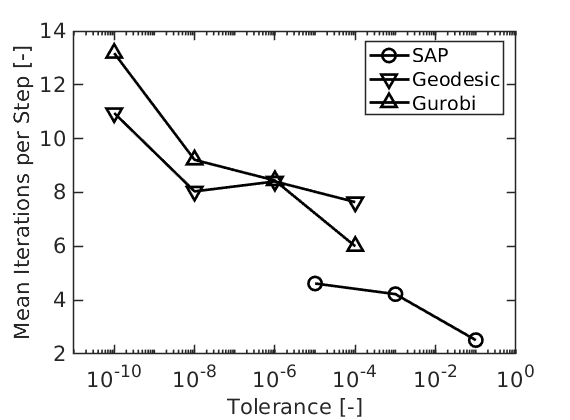
\includegraphics[width=0.7\columnwidth]{figures/dual_arm/iterations_per_step.png}
    \caption{\label{fig:dual_arm_iterations} Mean number of iterations per
    time-step for the dual arm simulation.}
\end{figure}

In summary, the simulation of this complex robotic task demonstrates how
accuracy translates directly to robustness. We observe how the maximum momentum
error defined in Eq. \eqref{eq:momentum_error} is a good proxy for robustness in
simulation; simulations with errors larger than about $10\%$ could not complete
the task successfully. In this regard, SAP provides a certificate of accuracy
that proves useful in practice.

